\subsection{Task 3}

As described in Section \ref{sec:task3intro}, several different cases of expansion have been studied and processed. For each case, streamlines have been plotted and pressure contours have been drawn. As expected, there is a drop in pressure after the fluid goes through the expansion. \\

\noindent Geometries and flows with different expansion ratios and their results are shown below. In each variation of the simulation, grid convergence have been checked to ensure meaningful results and interpretations. The converged element size was found at $10^{-3}$ meters. Also, residual parameters are verified to have reduced under tolerated values and the input and output fluxes are checked and verified to have the same magnitude (difference in fluxes are in the order of $10^{-9}$).\\

\noindent To compare the pressure differences using the equations \ref{eq:hm} and \ref{eq:headlosscoeff}, we can combine them and obtain the following formula which yields pressure difference from average velocity, density and K.

\begin{equation}
    \Delta p = \frac{K * V^2 * \rho}{2}
    \label{eq:final_dP}
\end{equation}

\subsubsection{Sudden and Moderate Expansion ($\frac{d}{D} = 0.6$)}

Using equation \ref{eq:final_dP}, the expected theoretical pressure drop can be calculated when K value is found from Figure \ref{fig:exp_plots} to be 0.4:

\[\Delta p = \frac{0.4 * 0.554^2 * 100}{2} = 6.138Pa \]


\noindent The red circles on Figure \ref{fig:06_locs} shows the locations of the probes used to take samples of pressures before and after the expansion. The value from the probe before the expansion is taken to be 32.7 Pa, while it is observed to have dropped to 26.1 Pa. This results in a $\Delta p$ of 6.6 Pa, which is \textbf{within 7.5\% error} of what is expected.

\begin{figure}[H]
    \centering
    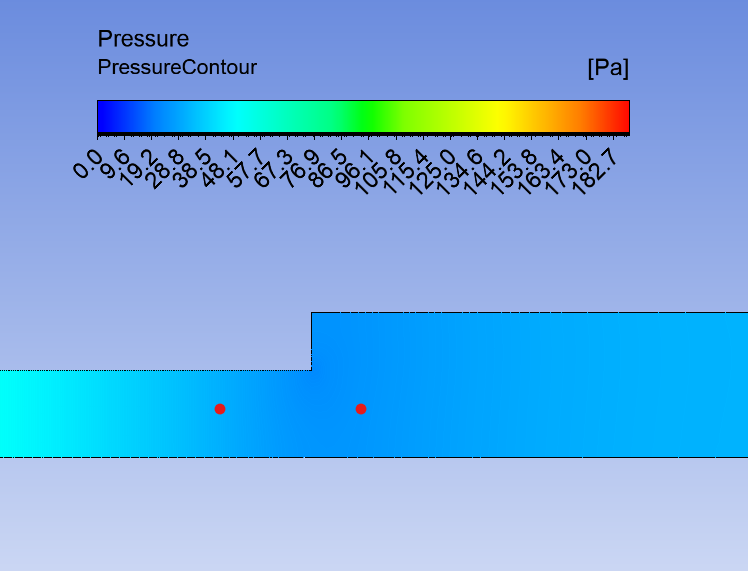
\includegraphics[width=.7\linewidth]{images/task3/06_locations.png}
    \caption{Pressure drop probe locations for moderate expansion}
    \label{fig:06_locs}
\end{figure}


\subsubsection{Sudden and Significant Expansion ($\frac{d}{D} = 0.4$)}

Using equation \ref{eq:final_dP}, the expected theoretical pressure drop can be calculated when K value is found from Figure \ref{fig:exp_plots} to be 0.7:

\[\Delta p = \frac{0.7 * 0.554^2 * 100}{2} = 10.74Pa \]


\noindent The red circles on Figure \ref{fig:04_locs} shows the locations of the probes used to take samples of pressures before and after the expansion. The value from the probe before the expansion is taken to be 20.2 Pa, while it is observed to have dropped to 8.9 Pa. This results in a $\Delta p$ of 6.6 Pa, which is \textbf{within 5.2\% error} of what is expected. Also, the streamlines for this case can be seen in Figure \ref{fig:04_stream}.

\begin{figure}[H]
\centering
\hfill
\begin{subfigure}{.48\textwidth}
    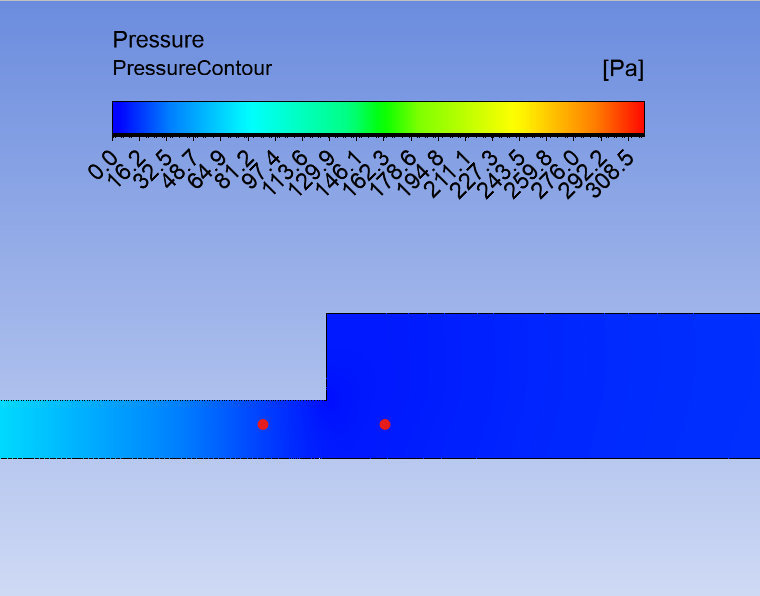
\includegraphics[width=.95\linewidth]{images/task3/04_locations.png}
    \caption{Pressure drop probe locations for significant expansion}
    \label{fig:04_locs}
\end{subfigure}
\hfill
\begin{subfigure}{.48\textwidth}
    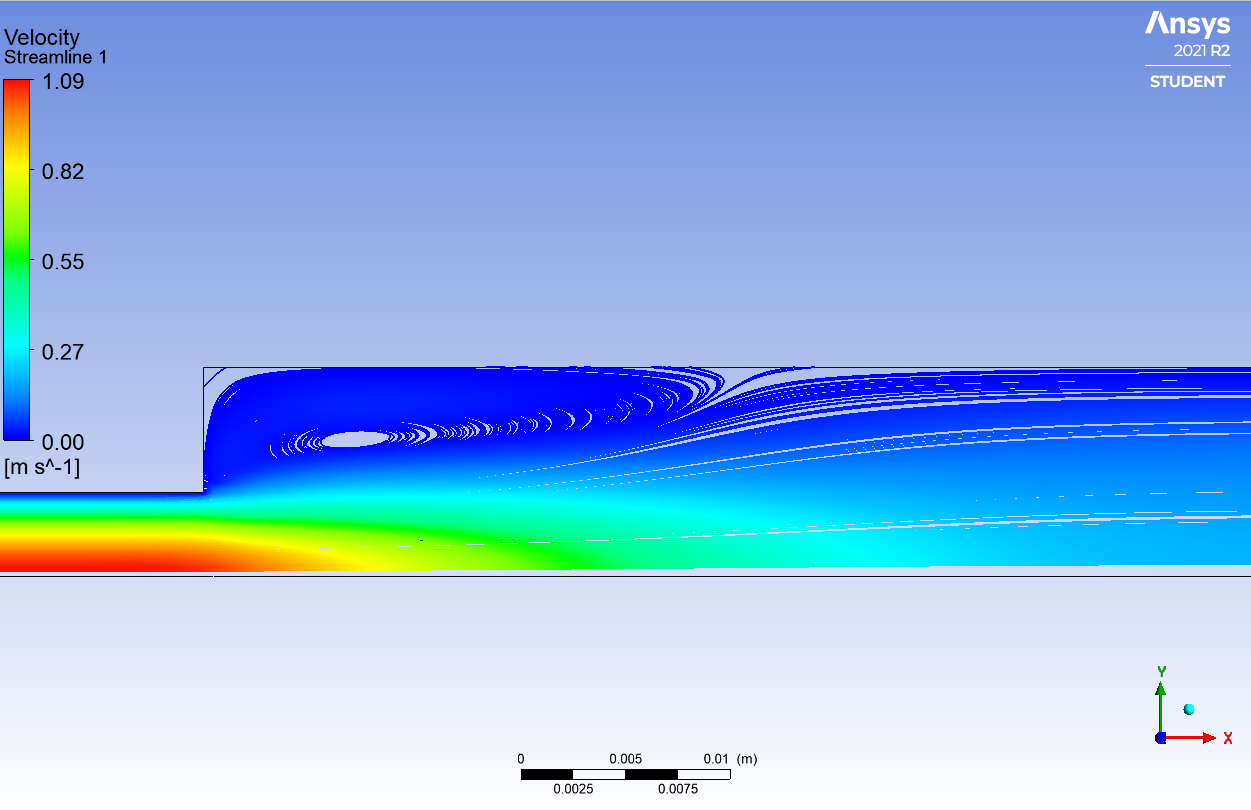
\includegraphics[width=.95\linewidth]{images/task3/04_streamlines.png}
    \caption{Streamlines for significant expansion}
    \label{fig:04_stream}
\end{subfigure}
\label{fig:04_figure}
\caption{Significant expansion pressure and streamlines}
\end{figure}


\subsubsection{Sudden and Severe Expansion ($\frac{d}{D} = 0.2$)}

Using equation \ref{eq:final_dP}, the expected theoretical pressure drop can be calculated when K value is found from Figure \ref{fig:exp_plots} to be 0.91:

\[\Delta p = \frac{0.91 * 0.554^2 * 100}{2} = 13.96Pa \]


\noindent The red circles on Figure \ref{fig:02_locs} shows the locations of the probes used to take samples of pressures before and after the expansion. The value from the probe before the expansion is taken to be 16.2 Pa, while it is observed to have dropped to 3.5 Pa. This results in a $\Delta p$ of 12.7 Pa, which is \textbf{within 9\% error} of what is expected. Also, the streamlines for this case can be seen in Figure \ref{fig:02_stream}.


\begin{figure}[H]
\centering
\hfill
\begin{subfigure}{.48\textwidth}
    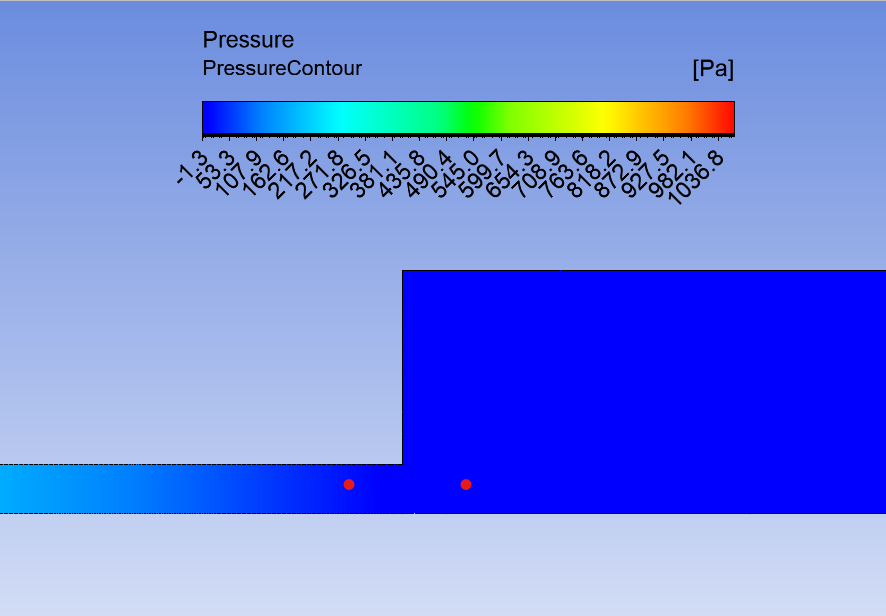
\includegraphics[width=.95\linewidth]{images/task3/02_locations.png}
    \caption{Pressure drop probe locations for severe expansion}
    \label{fig:02_locs}
\end{subfigure}
\hfill
\begin{subfigure}{.48\textwidth}
    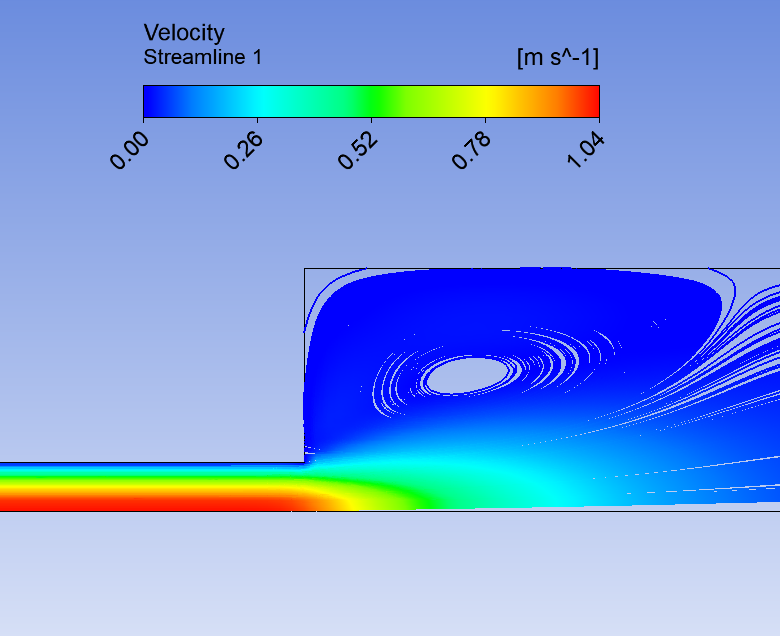
\includegraphics[width=.95\linewidth]{images/task3/02_streamlines.png}
    \caption{Streamlines for severe expansion}
    \label{fig:02_stream}
\end{subfigure}
\label{fig:02_figure}
\caption{Severe expansion pressure and streamlines}
\end{figure}


\subsubsection{Gradual and Moderate Expansion ($\frac{d}{D} = 0.4$)}

Using equation \ref{eq:final_dP}, the expected theoretical pressure drop can be calculated when K value is found from Figure \ref{fig:exp_plots} to be 0.91 (However, this time the plot for gradual expansion at a cone angle of $20^{\circ}$ is used):

\[\Delta p = \frac{0.38 * 0.554^2 * 100}{2} = 5.83Pa \]


\noindent The red circles on Figure \ref{fig:04_gradual_locs} shows the locations of the probes used to take samples of pressures before and after the expansion. The value from the probe before the expansion is taken to be 20.1 Pa, while it is observed to have dropped to 13.4 Pa. This results in a $\Delta p$ of 6.7 Pa, which is \textbf{within 13\% error} of what is expected. Also, the streamlines for this case can be seen in Figure \ref{fig:04_gradual_stream}. When examined, it can be clearly said that the gradual expansion did not induce a recirculation zone as it was observed for all sudden expansion cases, including tasks 1 and 2. Also, it causes less pressure drop when compared with sudden expansion for the same expansion ratio. The loss in pressure is lower in this case due to more laminar-like and less turbulent nature of the fluid inside the gradual expansion. The lack of recirculations affect the behavior and the properties of the fluid dearly.

\begin{figure}[H]
\centering

\begin{subfigure}{.48\textwidth}
    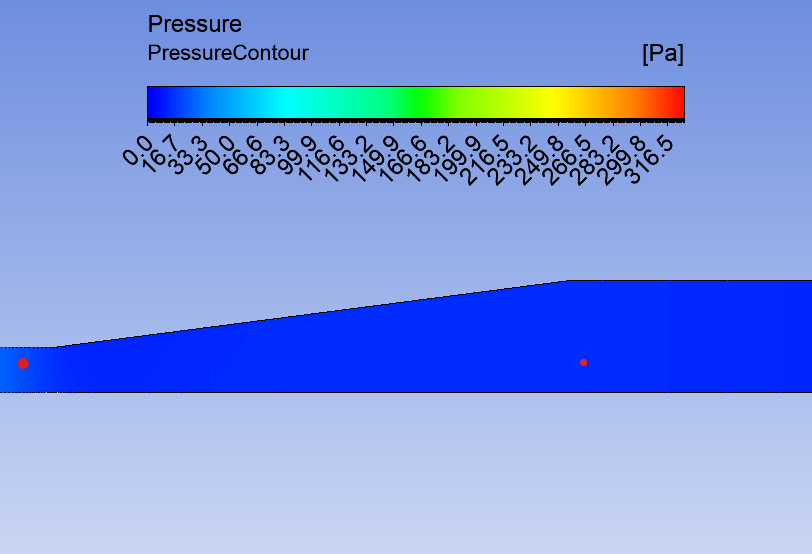
\includegraphics[width=.95\linewidth]{images/task3/04_gradual_locations.png}
    \caption{Pressure drop probe locations for gradual expansion}
    \label{fig:04_gradual_locs}
\end{subfigure}
\hfill
\begin{subfigure}{.48\textwidth}
    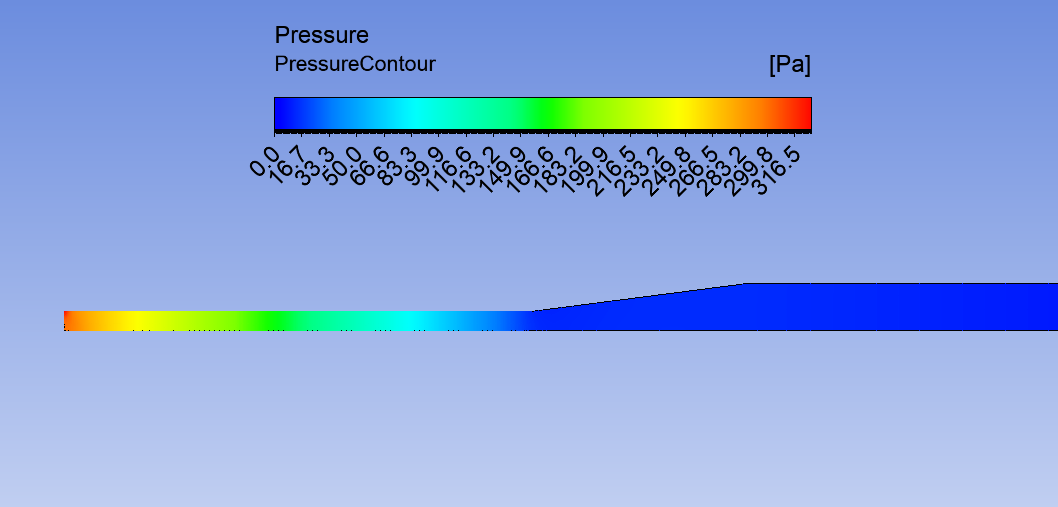
\includegraphics[width=.95\linewidth]{images/task3/04_gradual_press.png}
    \caption{Pressures for gradual expansion}
    \label{fig:04_gradual_pressure}
\end{subfigure}

\begin{subfigure}{.8\textwidth}
    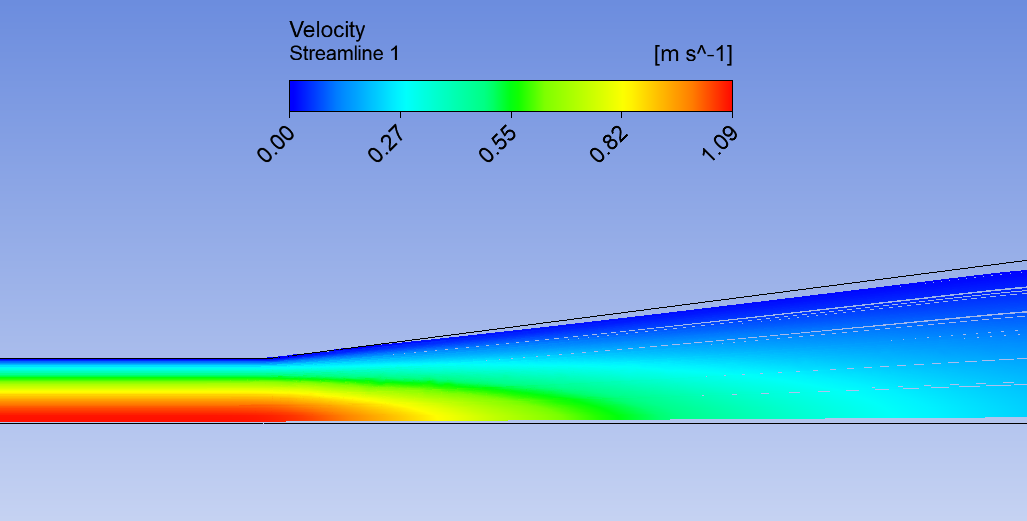
\includegraphics[width=.95\linewidth]{images/task3/04_gradual_streamlines.png}
    \caption{Streamlines for gradual expansion}
    \label{fig:04_gradual_stream}
\end{subfigure}

\label{fig:gradual_figure}
\caption{Gradual expansion pressure and streamlines and locations}
\end{figure}


\subsubsection{Optimization of the Expansion for $\frac{d}{D} = 0.5$}

As introduced in section \ref{sec:task3intro}, two different cases for expansion are studied. Among these two, for an expansion ratio of $0.5$, we have two options to choose, a sudden or a gradual expansion. The simulations and comparisons, along with equation \ref{eq:final_dP}, show that the smaller the K constant, the less pressure drop occurs. As can be seen from Figure \ref{fig:cone_angle}, the smallest K number that corresponds to 0.5 expansion ratio is found at a gradual expansion of around $7.6^{\circ}$. \\

\noindent Using those values, minimum K in estimated to be 2.5 which is shown in Figure \ref{fig:cone_angle}. Using that K value, the estimated pressure loss becomes:
\[\Delta p = \frac{0.25 * 0.554^2 * 100}{2} = 3.84Pa \]


\begin{figure}[H]
    \centering
    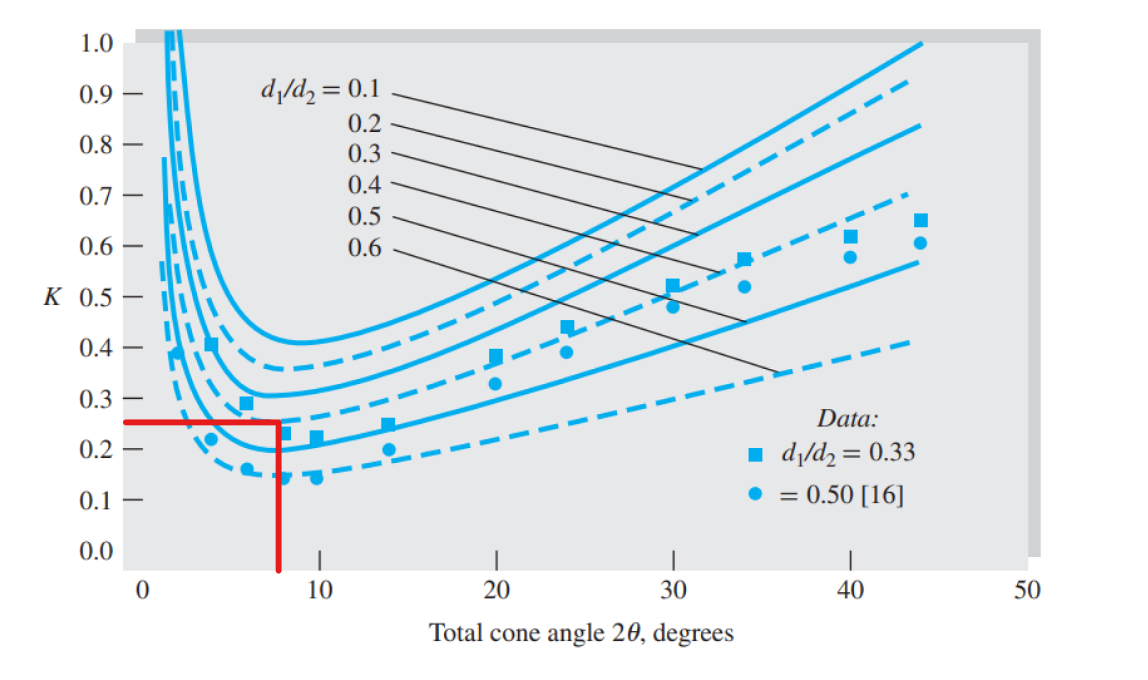
\includegraphics[width=.6\linewidth]{images/task3/cone_angle.png}
    \caption{Smallest K for a gradual expansion with a ratio of 0.5 \cite{white_chul_2016}}
    \label{fig:cone_angle}
\end{figure}


\noindent This 3.84Pa drop is the lowest observed during all previous expansion cases. Furthermore, according to the plot given by White's book, it is the lowest drop possible for 0.5 expansion ratio. The geometry has been modified to have a gradual expansion of said angle and the simulation has been run accordingly. The residuals, steady state conditions and grid convergence has been verified. The mesh independent results are plotted and can be seen from Figure \ref{fig:opt_figure}. 


\begin{figure}[H]
\centering

\begin{subfigure}{.48\textwidth}
    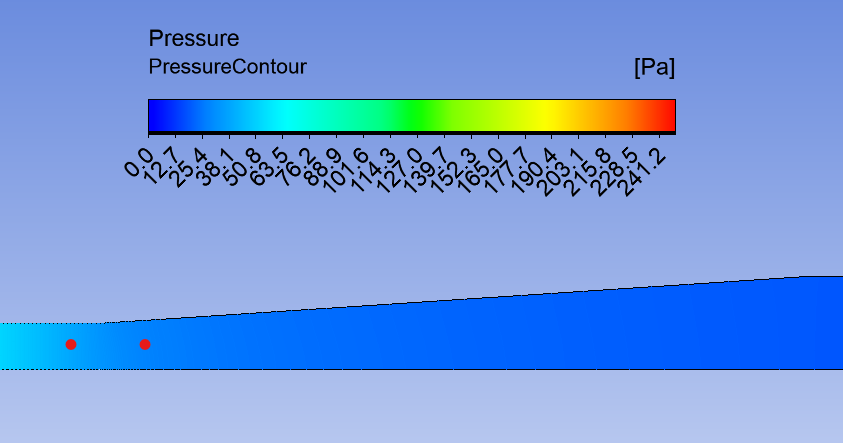
\includegraphics[width=.95\linewidth]{images/task3/optimized_locations.png}
    \caption{Pressure drop probe locations for optimized expansion}
    \label{fig:04_gradual_locs}
\end{subfigure}
\hfill
\begin{subfigure}{.48\textwidth}
    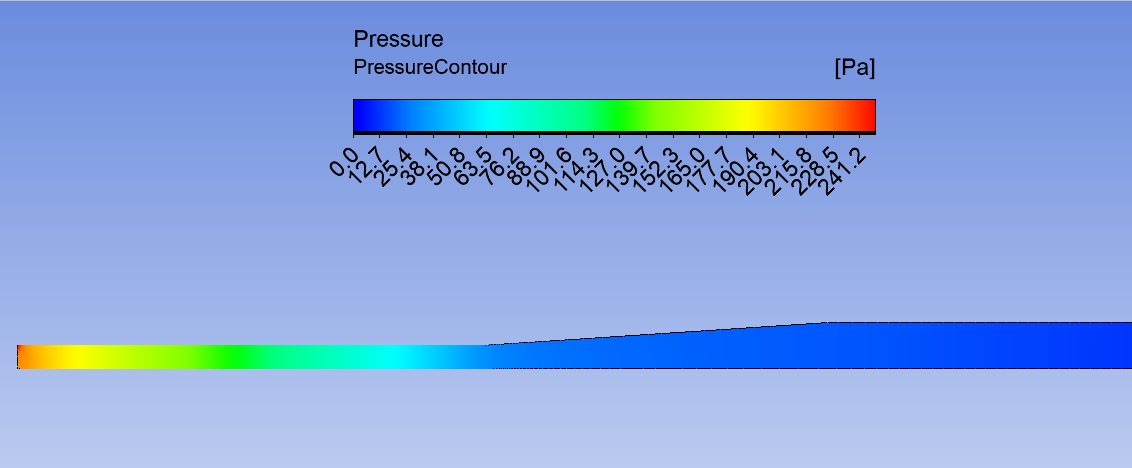
\includegraphics[width=.95\linewidth]{images/task3/optimized_pressure.png}
    \caption{Pressures for optimized expansion}
    \label{fig:04_gradual_pressure}
\end{subfigure}

\begin{subfigure}{.7\textwidth}
    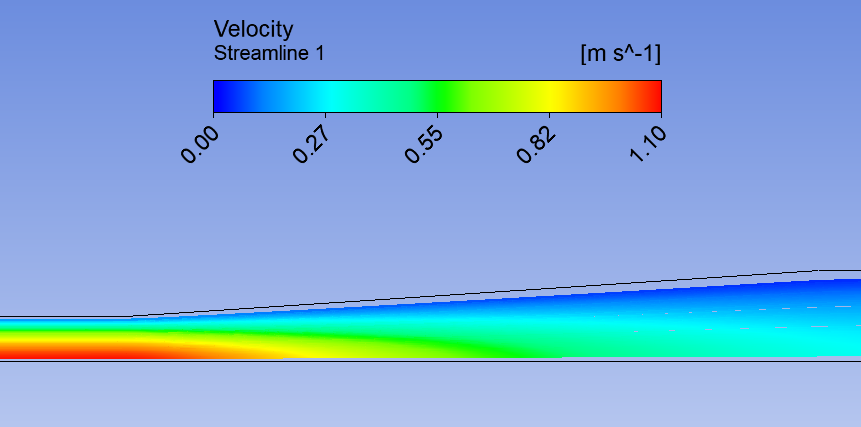
\includegraphics[width=.95\linewidth]{images/task3/optimized_streamline.png}
    \caption{Streamlines for optimized expansion}
    \label{fig:04_gradual_stream}
\end{subfigure}

\caption{Optimized expansion pressure and streamlines and locations}
\label{fig:opt_figure}
\end{figure}



\noindent To sum up, it can be said that with the data we have in our disposal, \textbf{a gradual expansion with a cone angle of 7.6 degrees} is the optimum setup for minimum pressure loss caused by the expansion.
